\documentclass[handout, usenames,dvipsnames, nosymbols,aspectratio=169]{beamer}

\usepackage[ngerman]{babel}		% German headings.
\usepackage[T1]{fontenc}			% German typesetting.
\usepackage[utf8]{inputenc} 		%Universal/Linux Kodierung

\usepackage{lmodern}				% Better font encoding.
\usepackage{amsmath, amsfonts, amssymb, amsxtra} % Mathematical symbols.
\usepackage{geometry}
\usepackage{graphicx}
\usepackage{subfigure}
\usepackage{tikz}
\usepackage[german, useregional]{datetime2}

\beamertemplatenavigationsymbolsempty	% Slices without navigation symbols.

\usepackage{xcolor}

% doc informations
\DTMsavedate{docdate}{2024-03-16}
\newcommand{\docplace}{Magdeburg}

\newcommand{\netzlogo}{include/netz39_logo_web_light.png}

\newcommand{\docauthor}{Maximilian Grau}
\newcommand{\doctitle}{Punktschweißen -- Workshop}
\newcommand{\docsubtitle}{}

\newcommand{\mainColor}{BurntOrange}
\usecolortheme[named=\mainColor]{structure}
				% edit here author informations.

\renewcommand{\titlepage}
{
\begin{frame}[plain]
	\begin{tikzpicture}[remember picture,overlay]
		\fill[darkgray] (current page.north west) rectangle ++(\paperwidth,-0.3\paperheight);
		\node[\mainColor, yshift=-0.15\paperheight, font=\Huge] at (current page.north) {\doctitle};
		\node[gray, yshift=0.1\paperheight, font=\Large] at (current page.center) {\docauthor};
		\node[gray, yshift=-0.0\paperheight, font=\normalsize] at (current page.center) {\DTMusedate{docdate}};
		\node[yshift=0.225\paperheight] at (current page.south) {\includegraphics[height=0.35\paperheight]{\netzlogo}};
	\end{tikzpicture}
\end{frame}
}
\setbeamertemplate{headline}% Headings
{
	\hspace*{0.02\textwidth}
	\begin{minipage}[m]{0.3\textwidth}
		\vspace*{1ex}
		\includegraphics[height=8mm]{\netzlogo}
	\end{minipage}
	\begin{minipage}[m]{0.35\textwidth}
		\centering
		\vspace*{3ex}
		\doctitle
	\end{minipage}
	\hfill
	\begin{minipage}[m]{0.14\textwidth}
		\vspace*{3ex}
		 \hfill Folie:  \insertframenumber ~ / \inserttotalframenumber
		\hspace*{0.1\textwidth}
	\end{minipage}
	\color{\mainColor}
	\rule{\paperwidth}{1pt}
}
%
%
%
\setbeamertemplate{footline} % Footer
{
	\color{\mainColor }
	\rule{\paperwidth}{1pt}
	\color{black}
	\begin{minipage}[c]{\textwidth}
		\vspace*{1ex}
		\hspace*{0.02\textwidth} \docauthor \hfill  \DTMusedate{docdate} \hspace{0.02\textwidth}
		\vspace*{2ex}
	\end{minipage}
}

\begin{document}

	\addtocounter{framenumber}{-1}	% exclude title page from pagecounter.
	\titlepage
	
	\begin{frame}
		\frametitle{Ziele des Workshops}
		\begin{itemize}[<+->]
			\item Grundlagen des Punktschweißens
			\item Bedienung des Schweißgerätes
			\item praktische Übungen
			\item Umgang mit 18650-Zellen
		\end{itemize}
	\end{frame}
	
	\begin{frame}
		\frametitle{Was ist Punktschweißen?}
		Punktschweißen nutzt das Prinzip des \textbf{Widerstandsschweißens}\\[0.5em]
		\begin{minipage}{0.65\textwidth}	
			\begin{itemize}[<+->]
				\item elektrischer Strom wird angelegt
				\item an den zu schweißenden Punkten auf dem Metall herrscht ein hoher Widerstand
				\item  ${W_{s} = I^{2}_{s}R_{s}t_{s}}$\\
				\color{gray}
				$W_{s}$ - Schweißenergie | $I_{s}$ - Strom | $t_{s}$ - Schweißzeit\\
				$R_{s}$ - Widerstand an der Schweißstelle\\
				\normalcolor
				\item enorme Erhitzung $\rightarrow$ Metall schmilzt
				\item durch Druckausübung bilden beide Metalle bei Abkühlung an diesem Punkt eine feste Verbindung
			\end{itemize}
		\end{minipage}
		\begin{minipage}{0.3\textwidth}
			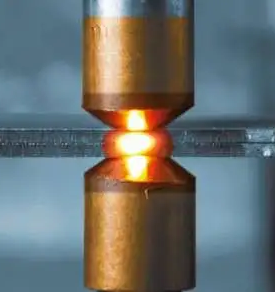
\includegraphics[width=\textwidth]{images/Copper-electrodes-create-a-spot-weld.png}
			\tiny
			{\color{gray}\url{https://proleantech.com/spot-welding-advantages-disadvantages-application}}
		\end{minipage}
		
	\end{frame}
	
	\begin{frame}
		\frametitle{Punktschweißgerät im Netz39\,e.V.}
		\begin{minipage}{0.5\textwidth}	
			\begin{itemize}
				\item \textbf{kWeld} von keenlab
				\item bis zu 500\,Joule bzw. 2000\,Ampere
				\item Steuerung über LCD und Drehknopf
				\item Schweißen geschieht entweder über Fußpedal oder Automatik
				\item Anschluss an Ultrakondensatoren oder LiPo-Akku
			\end{itemize}
		\end{minipage}
		\begin{minipage}{0.45\textwidth}
			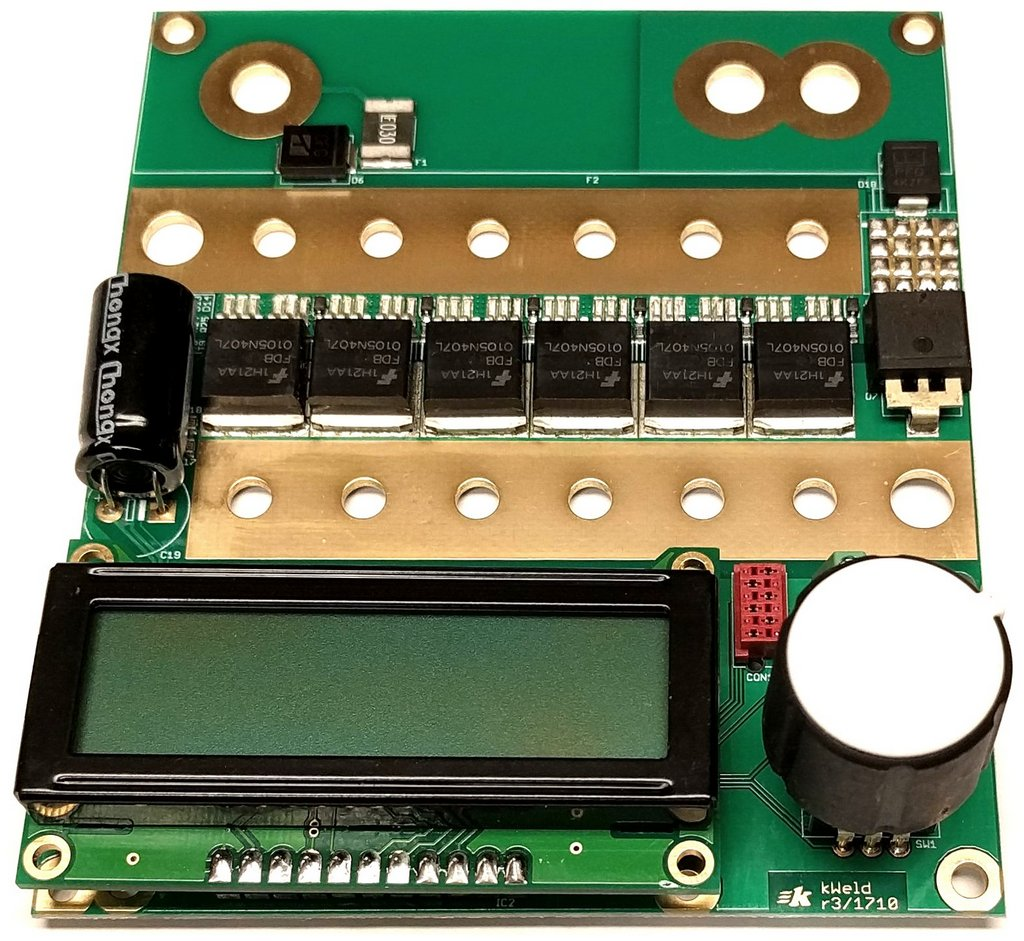
\includegraphics[width=\textwidth]{images/kWeld-electronics.jpg}
			\tiny
			{\color{gray}\url{https://www.keenlab.de/index.php/product/kweld-electronics/}}
		\end{minipage}
	\end{frame}
	
	\begin{frame}
		\frametitle{Anforderungen an die Spannungsquelle:}
		Damit ein sehr hoher Strom fließen kann, brauchen wir eine Spannungsquelle mit einem sehr niedrigen Innenwiderstand. Die zwei einfachsten Möglichkeiten sind:\\[2em]
		\hfill
		\begin{minipage}{0.45\textwidth}
			\onslide<2->\textbf{Ultrakondensatoren}\\[0.5em]
			\onslide<2->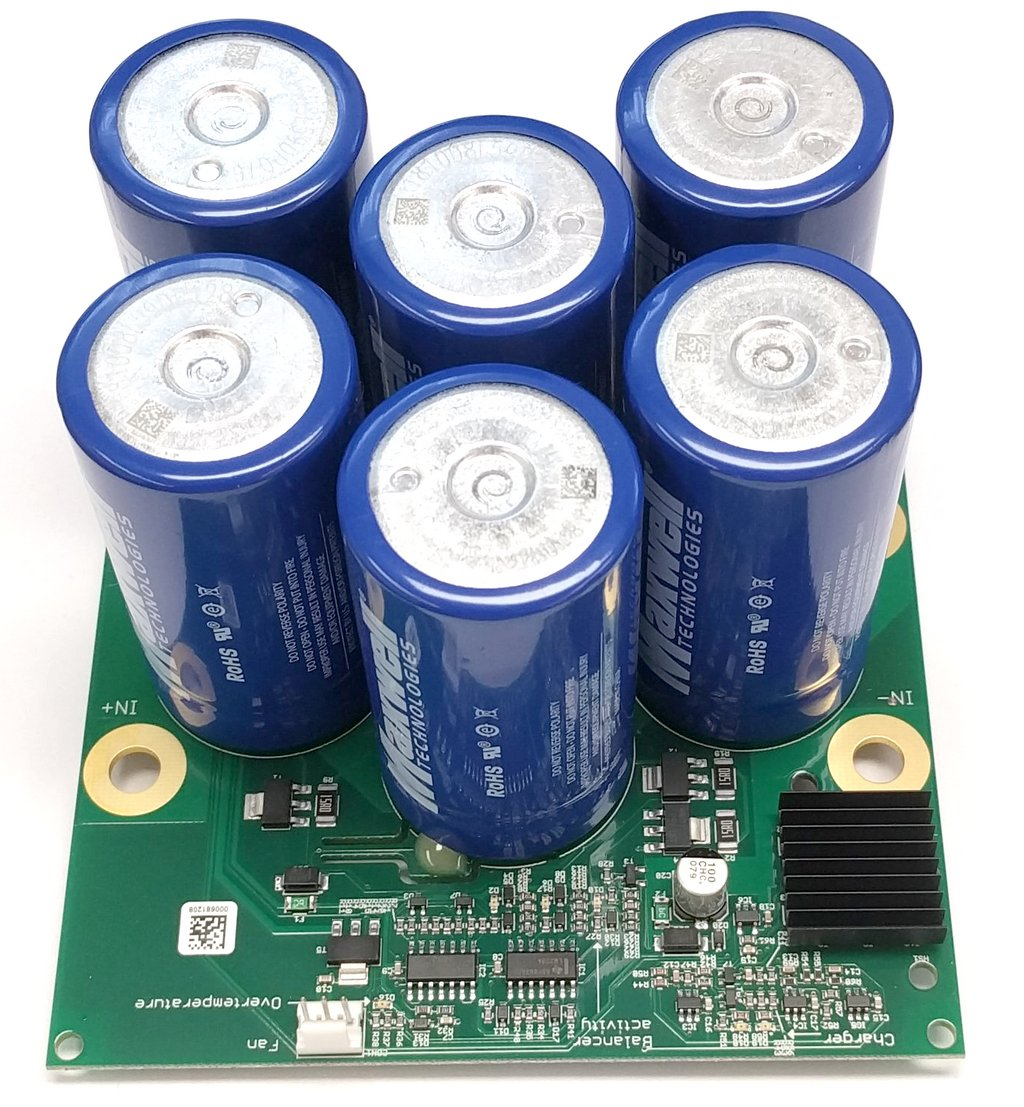
\includegraphics[width=0.55\textwidth]{images/kCap-r4-3.jpg}\\
			\tiny
			\onslide<2->{\color{gray}\url{https://www.keenlab.de/index.php/product/kweld-ultracapacitor-module/}}
		\end{minipage}
		\hspace{1em}
		\begin{minipage}{0.45\textwidth}	
		    \onslide<3->\textbf{Lithium-Polymer (LiPo-Akku)}\\[1.5em]
			\onslide<3->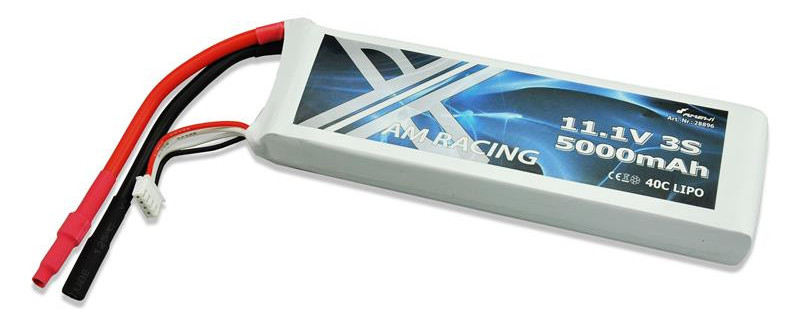
\includegraphics[width=\textwidth]{images/lipo.jpg}\\[1.5em]
			\tiny
			\onslide<3->{\color{gray}\url{https://spielzeug-fuchs.de/produkt/lipo-akku-3s-111v-5000mah-40c-softcase-5mm-goldkontakt/}}
		\end{minipage}
	\end{frame}

	\begin{frame}
		\frametitle{Arbeitsschutz}
		Gefahren beim Schweißen entstehen durch:\\[0.5em]
		\begin{itemize}[<+(1)->]
			\item Funkenbildung aufgrund herausgespritztem schmelzflüssigem Schweißgut
			\item überhitzten LiPo-Akku
			\item starke magnetische Felder
		\end{itemize}
		\vfill
		\begin{minipage}{0.475\textwidth}
			\centering
			\onslide<5->
\includegraphics[width=0.4\textwidth]{images/ISO_7010_P007.png}\\
			\footnotesize
			\onslide<5->Verbot für Personen mit \\
			\onslide<5->Herzschrittmacher nach ISO 7010\\
			\tiny
			\onslide<5->{\color{gray}\url{https://commons.wikimedia.org/w/index.php?curid=26500071}}
		\end{minipage}
		\begin{minipage}{0.475\textwidth}
			\centering
			\onslide<5->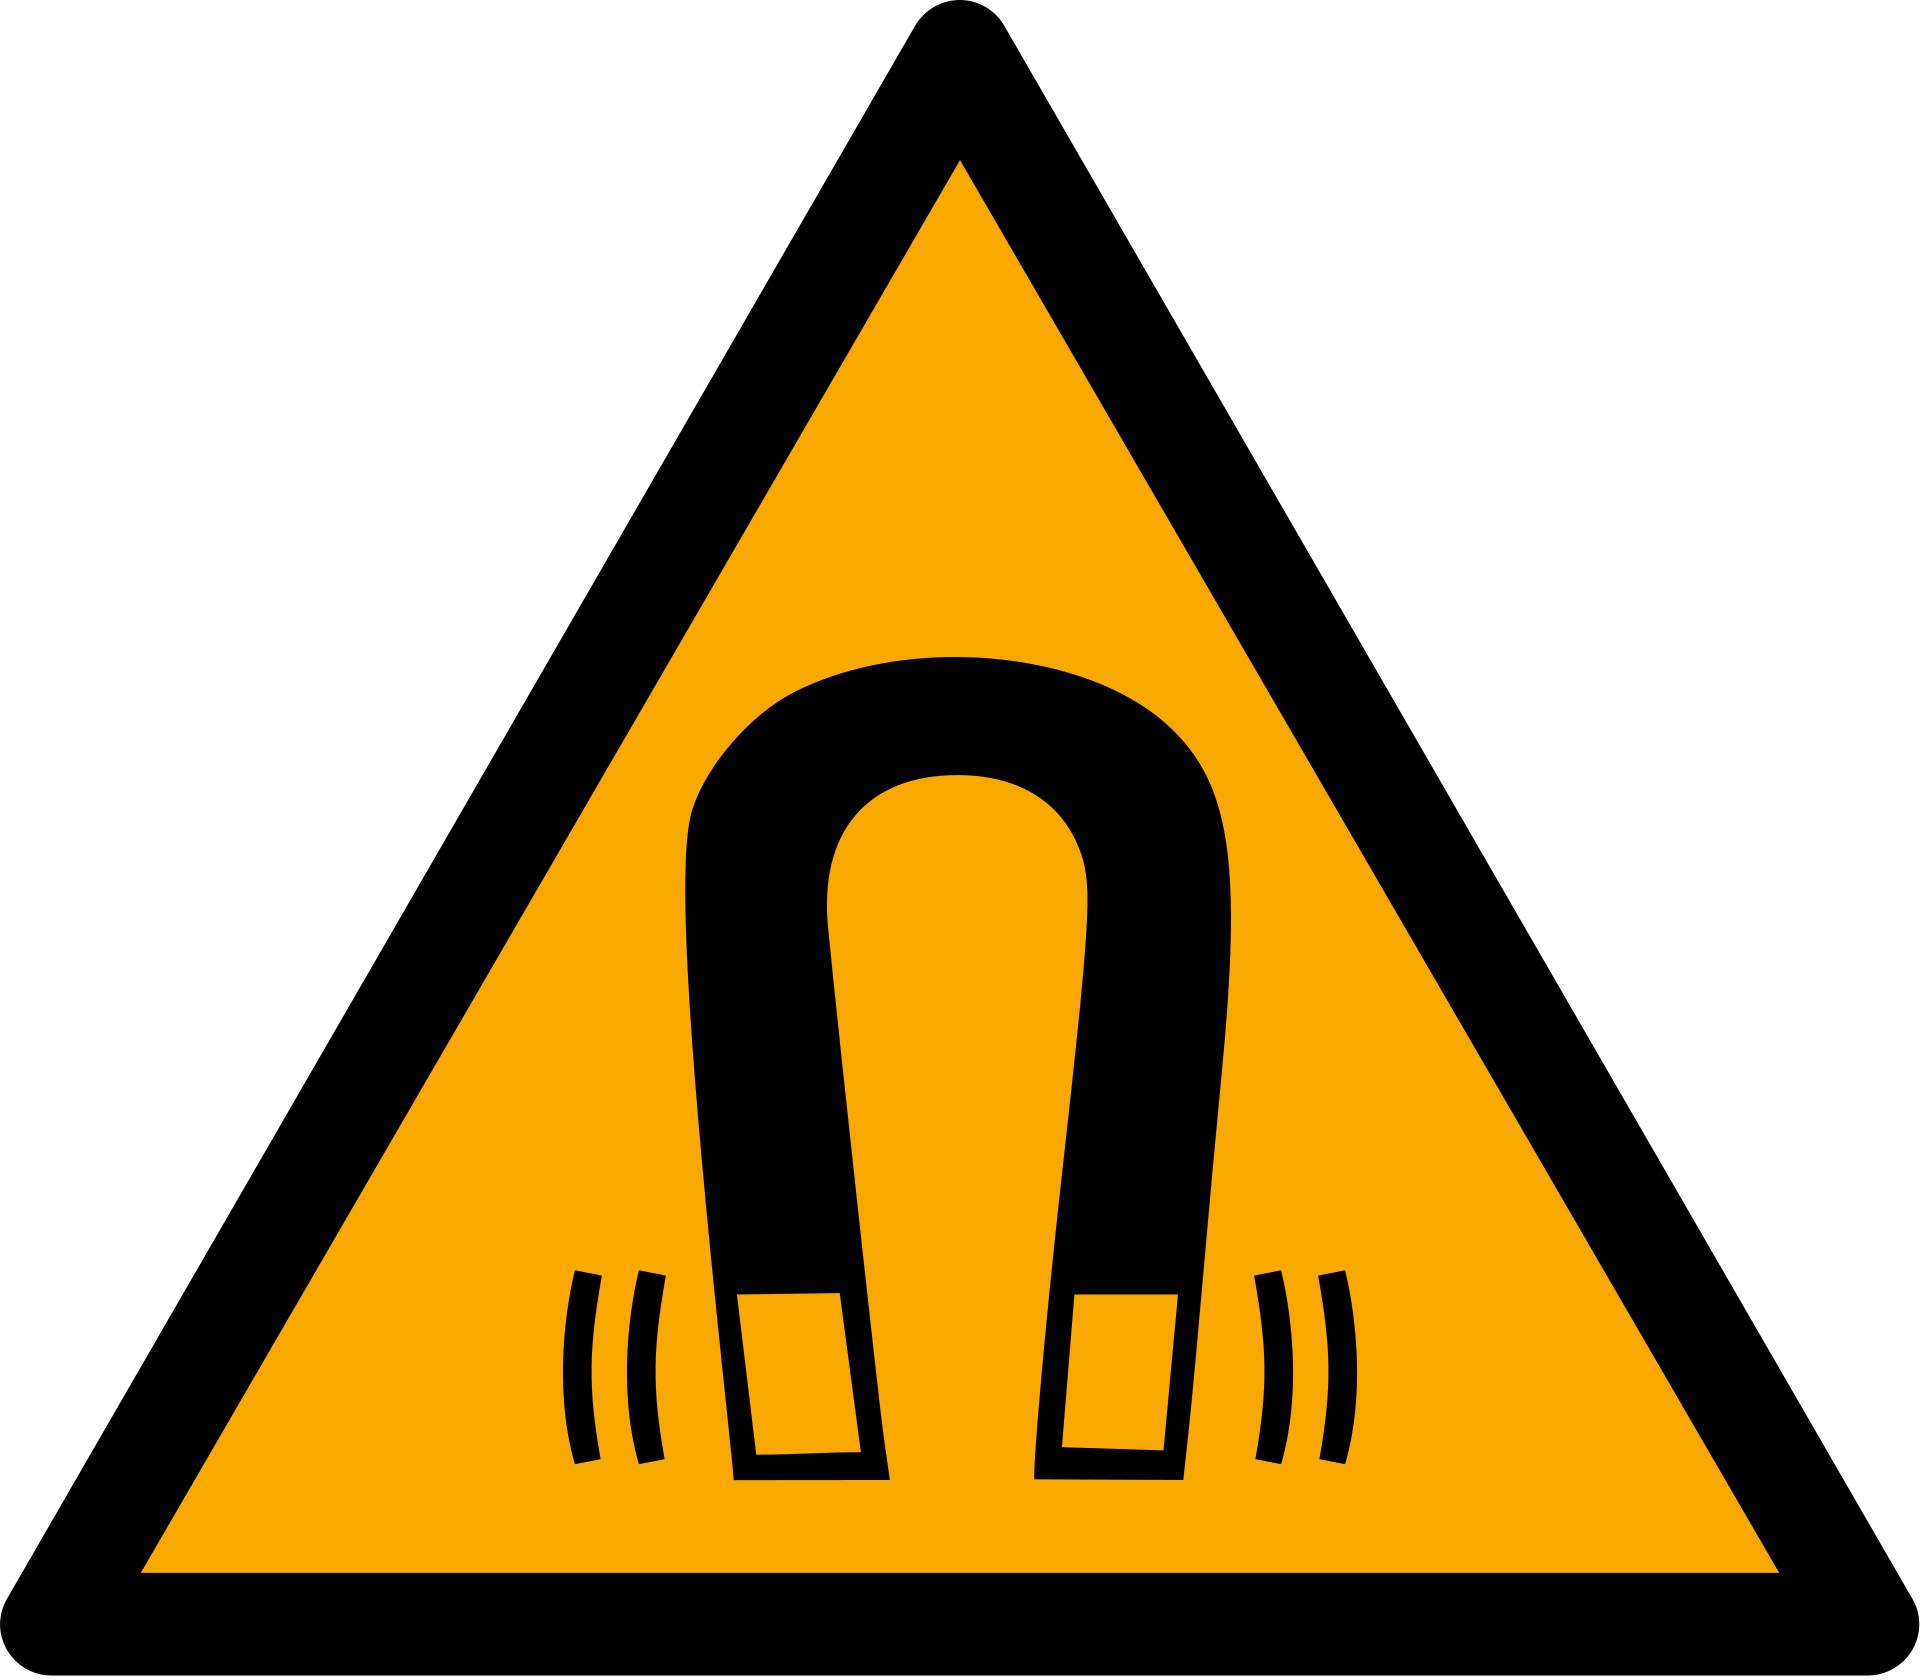
\includegraphics[width=0.45\textwidth]{images/ISO_7010_W006.png}\\
			\footnotesize
			\onslide<5->Warnung vor magnetischem  \\
			\onslide<5->Feld nach ISO 7010\\
			\tiny
			\onslide<5->{\color{gray}\url{https://commons.wikimedia.org/w/index.php?curid=26501573}}
		\end{minipage}		
	\end{frame}
	
	\begin{frame}
		\frametitle{Materialwahl}
		\textbf{Elektrodenmaterial:}
		\begin{itemize}
			\item bestehen aus Kupfer
			\item hohe Wärmeleitfähigkeit, sehr geringer elektr. Widerstand
		\end{itemize}
		%
		\onslide<2->$\rightarrow$ Wärme wird dadurch vorzugsweise in Werkstücken, nicht in Elektroden, erzeugt
		\\[1em]
		\onslide<3->\textbf{Materialien zum Punktschweißen:}
		\begin{itemize}
			\onslide<3->\item Edelstahl
			\onslide<3->\item (verzinkter) Stahl
			\onslide<3->\item Nickellegierungen
			\onslide<3->\item Titan
		\end{itemize}
		\onslide<4->Alle leiten Wärme schlecht und besitzen einen hohen elektr. Widerstand\\
		\onslide<4->$\rightarrow$ geeignete Materialien zum Punktschweißen
	\end{frame}
	
	\begin{frame}
		\frametitle{Joule-Einstellung}
		Die Menge an Energie, die für das Erstellen von Schweißpunkten fließen muss, hängt vom Material und dessen Dicke ab.\\[2em]
		\begin{center}
		\begin{tabular}{| c | c|}
			
			\hline
			dünner Nickelstreifen (0,15\,mm) & 20-25\,J \\ 
			\hline
			dicker Nickelstreifen (0,25\,mm) & 30-40\,J \\  
			\hline 
		\end{tabular}
		\end{center}
	\end{frame}
	
	\begin{frame}%<handout:0>
		\frametitle{Gefährlichkeit von Spannung/Strom}
		Welche Konstellation ist gefährlich für den menschlichen Körper?\\[1em]
		Der Mensch fässt eine Leitung an, dort liegt eine Spannung an und es fließt ein Strom.\\[1em]
		\hfill
		\begin{minipage}{0.4\textwidth}
			\textbf{Konstellation 1:}\\
			Spannung: 16\,V\\
			Strom: 1600\,A\\
		\end{minipage}
		\hspace{2em}
		\begin{minipage}{0.4\textwidth}
			\textbf{Konstellation 2:}\\
			Spannung: 1600\,V\\
			Strom: 50\,mA\\
		\end{minipage}
	\end{frame}
	
	\begin{frame}<handout:0>
		\frametitle{Praxis}
		\centering\Large
		Nun wird geschweißt!
	\end{frame}
	
	\begin{frame}
		\frametitle{Umgang mit 18650-Zellen}
		Kurzschluss-Gefahr ist hoch -- nicht hebeln beim Entfernen von Nickelstreifen!\\[1em]
		\begin{minipage}{0.3\textwidth}
			\centering
			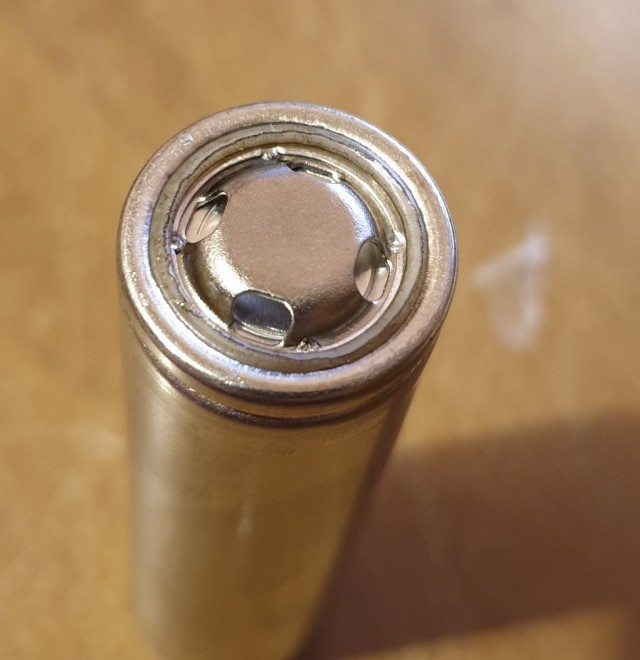
\includegraphics[width=0.8\textwidth]{images/18650_naked.jpg}\\
			\textbf{+} und \textbf{-} sind sich\\
			gefährlich nahe
		\end{minipage}
		\begin{minipage}{0.35\textwidth}
			\centering	
			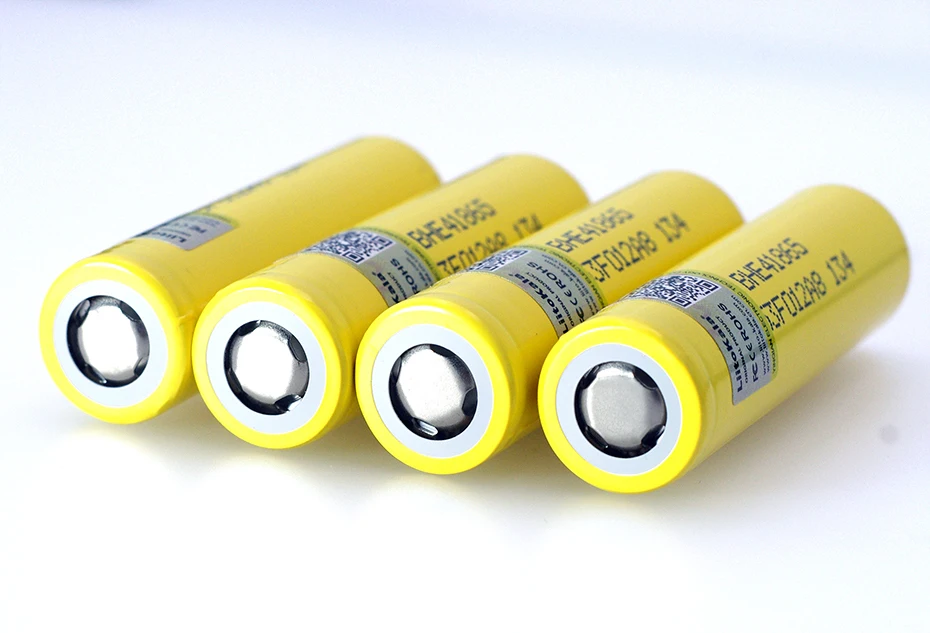
\includegraphics[width=0.8\textwidth]{images/18650_normal.png}\\
			Werkszustand: gelber\\
			Schrumpfschlauch und weißer Isolationsring)
		\end{minipage}
		\begin{minipage}{0.3\textwidth}
			\centering
			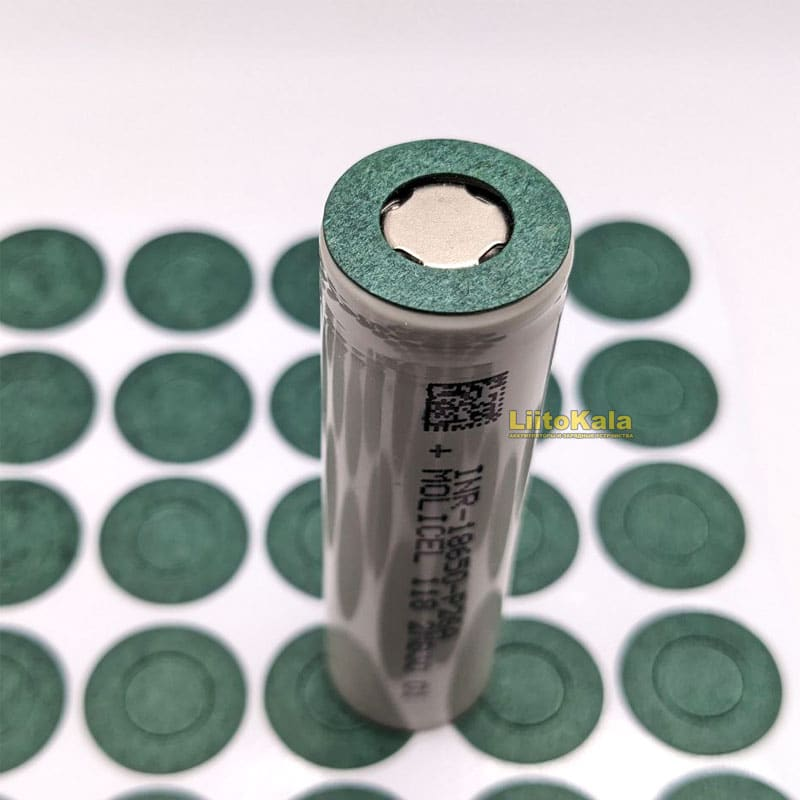
\includegraphics[width=0.8\textwidth]{images/isolated-ring-18650-2.jpg}\\
			zusätzlicher Isolationspad
		\end{minipage}
	\end{frame}
	
	\begin{frame}
		\frametitle{Umgang mit 18650-Zellen}
		Alte Schweißpunkte mit Dremel glatt schleifen.\\ Nur so können qualitativ gute neue Schweißpunkte entstehen.\\[1em]
		\hspace{2em}
		\begin{minipage}{0.4\textwidth}
			\centering
			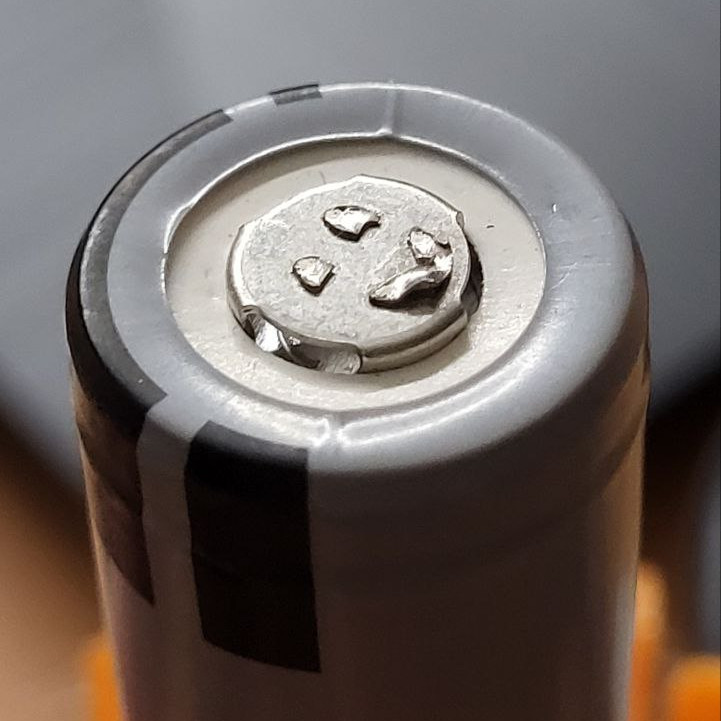
\includegraphics[width=0.75\textwidth]{images/photo_2024-03-16_01-08-52.jpg}\\
			alte Schweißpunkte auf einer 18650-Zelle	
		\end{minipage}
		\hspace{1em}
		\begin{minipage}{0.4\textwidth}
			\centering
			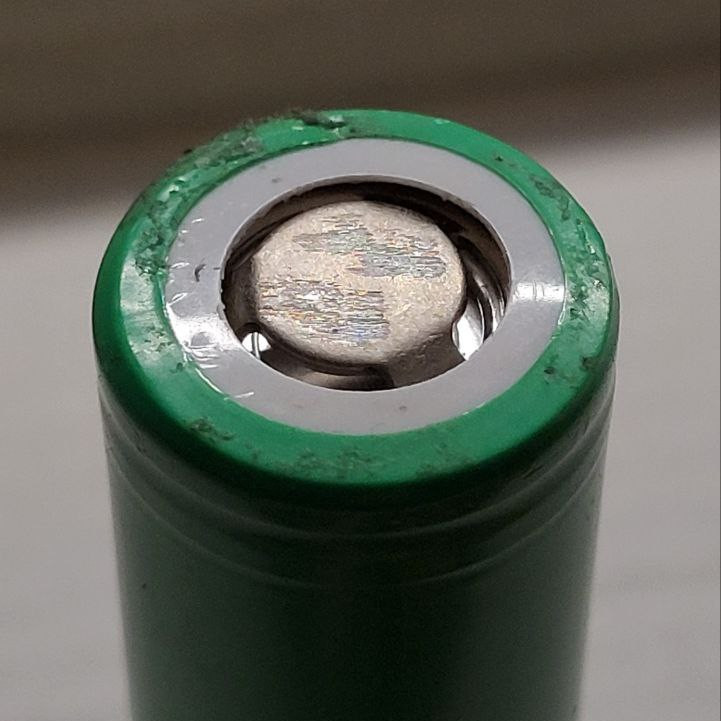
\includegraphics[width=0.75\textwidth]{images/photo_2024-03-16_01-08-55.jpg}\\
			glatt geschliffene Oberfläche\\
			\vfill
		\end{minipage}
	\end{frame}
	
	\begin{frame}
	\frametitle{Wartung}
	 \textbf{ Kupferelektroden neu anspitzen:}\\[0.5em]
	  \begin{minipage}{0.5\textwidth}
		  \begin{itemize}
		  	\item Schrauben lösen, Elektrode entnehmen
		  	\item Elektrode in die Tischbohrmaschine einspannen
		  	\item mit feinem Sandpapier die Spitze anschleifen, bis sie wieder blank und einigermaßen spitz ist
		  \end{itemize}
	 	\textbf{LiPo-Akku wieder auf \\Storage-Spannung laden}
	  \end{minipage}
	  \hfill
	  \begin{minipage}{0.4\textwidth}
	  	 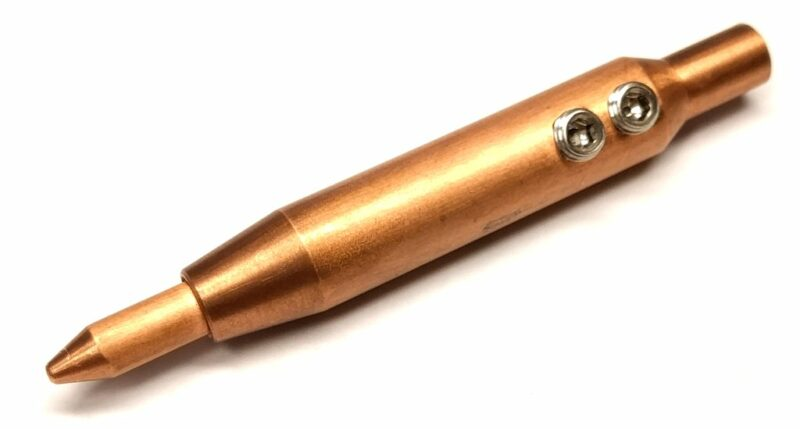
\includegraphics[width=\textwidth]{images/kWeld-new-electrodes-800x429.jpg}
	  	 \tiny
	  	 {\color{gray}\url{https://www.keenlab.de/index.php/product/kweld-electronics/}}
	  \end{minipage}
	\end{frame}


\end{document}